\documentclass[12pt]{article}
\usepackage[english]{babel}
\usepackage{lipsum}
\usepackage[square, numbers]{natbib}
\bibliographystyle{plainurl}
\usepackage{url}
\usepackage[utf8x]{inputenc}
\usepackage{amsmath}
\usepackage{mathtools}
\usepackage{mathtools,siunitx}
\sisetup{detect-all}
\usepackage{graphicx}
\graphicspath{{images/}}
\usepackage{parskip}
\usepackage{fancyhdr}
\usepackage{vmargin}
\usepackage{hyperref}
\usepackage{todonotes}
\usepackage{textcomp}
\usepackage{float}
\usepackage{listings}
\usepackage{enumitem}
\usepackage{caption}
\usepackage{listings}


\usepackage{color} %red, green, blue, yellow, cyan, magenta, black, white
\definecolor{mygreen}{RGB}{28,172,0} % color values Red, Green, Blue
\definecolor{mylilas}{RGB}{170,55,241}
\setmarginsrb{2 cm}{2.5 cm}{2 cm}{2.5 cm}{1 cm}{1 cm}{1 cm}{1 cm}
\presetkeys{todonotes}{fancyline}{}



%%%%%%%%%%%%%%%%%%%%%%%%%% TITLE %%%%%%%%%%%%%%%%%%%
\title{Image \& Signal Processing}
\author{A. Scharf, A. Wenzel}	
\date{\today}

\makeatletter
\let\thetitle\@title
\let\theauthor\@author
\let\thedate\@date

\providecommand\add@text{}
\newcommand\tagaddtext[1]{%
  \gdef\add@text{#1\gdef\add@text{}}}% 
\renewcommand\tagform@[1]{%
  \maketag@@@{\llap{\add@text\quad}(\ignorespaces#1\unskip\@@italiccorr)}%
}
\makeatother

\pagestyle{fancy}
\fancyhf{}
\rhead{\theauthor}
\lhead{\thetitle}
\cfoot{\thepage}

%% Uncomment the following line if subsections shall be numbered with alphabetic characters instead of numbers!
%\renewcommand{\thesubsection}{\thesection.\alph{subsection}}



\begin{document}

\lstset{language=Matlab,%
    %basicstyle=\color{red},
    breaklines=true,%
    morekeywords={matlab2tikz},
    keywordstyle=\color{blue},%
    morekeywords=[2]{1}, keywordstyle=[2]{\color{black}},
    identifierstyle=\color{black},%
    stringstyle=\color{mylilas},
    commentstyle=\color{mygreen},%
    showstringspaces=false,%without this there will be a symbol in the places where there is a space
    numbers=left,%
    numberstyle={\tiny \color{black}},% size of the numbers
    numbersep=9pt, % this defines how far the numbers are from the text
    emph=[1]{for,end,break},emphstyle=[1]\color{red}, %some words to emphasise
    %emph=[2]{word1,word2}, emphstyle=[2]{style},
}

%%%%%%%%%%%%%%%%%%%% Titlepage start %%%%%%%%%%%%%%%%%%%%%%%%%%%%

\begin{titlepage}
	\centering
    \vspace*{0.5 cm}
    
\includegraphics[scale = 0.15]{images/upslogo}\\[1.0 cm]

	\textsc{\Large M2 - TSI}\\[0.5 cm]

	\textsc{\large UE34 Laboratory Report}\\[0.5 cm]	
	\vspace{1cm}
	\rule{\linewidth}{0.2 mm} \\[0.4 cm]
	{ \huge \bfseries \thetitle}\\
	\rule{\linewidth}{0.2 mm}
	\\[0.5cm]
		\textsc{}
		\\[2.5 cm]

	\vspace{1cm}
	\emph{Authors:}\\
	Arthur Scharf\\
	Andreas Wenzel
	\vspace{2cm}
	
	{\large \today }\\[2 cm]
 
	\vfill
	
\end{titlepage}
%%%%%%%%%%%%%%%%%%% Titlepage end %%%%%%%%%%%%%%%%%%%%%%%%%%%%%%%


%%%%%%%%%%%%%%%%% include content %%%%%%%%%%%%%
%%%%%%%%%%%%%%%%% TASK 1 %%%
\section{Introduction - Image Processing for Earth Observation}
Image processing and the analysis of image data plays an important role especially for Earth Observations, but also in other fields related to space applications that make use of images, e.g. optical navigation or optical attitude control systems. In this report, we present a thorough overview of examples for image processing techniques, especially applying examples in Matlab. We focus on colour spaces for images, fourier transforms of basic figures, erosion and delatation and classification. 

\subsection{Computer Vision}
From a mathematical point of view, an image is an application that associates a value $I(u,v)$ to a pixel $(u,v)$. Pixels are atomic elements arranged in rows and columns,  such that the size of an image is given by the number of rows and the number of columns. Therefore, an image can be processed by using a matrix representation, where each matrix element $(u,v)$  represents a pixel containing the value $I(u,v)$ of the pixel.. In the case of multispectral images, i.e. colour images like RGB images (see following chapter), an image is an application that associates saveral values, e.g. $I_{1}(u,v)$ $I_{2}(u,v)$ and $I_{3}(u,v)$ to a pixel $(u,v)$, where the values $I_{i}$ represent a different colour like red, green and blue in RGB images. Therefore, each matrix element $(u,v)$ contains a vector of values. This matrix notation is the basic of image processing using Matlab.

\section{Greyscale and Colour images}
The understanding of colour images and the connection to their greyscale representation are fundamental for image analysis and image processing. We illustrate colour images in this section by  considering the examples of RGB and HSV colour space. There are also other colour spaces like CYMK (cyan, yellow, magenta, black) or YUV, but we only consider the first two in our examples since these are the most frequently used ones and essential for the understanding of coloured images. CYMK and YUV are mainly based on the first two colour spaces.

\subsection{Greyscale Images}
Greyscale images are basic images where the value of each pixel e.g. is associated to a value between 0, which is black, to 1 for bright. An example including an optical illusion is presented in image \ref{fig:greyillusion}. For this image, a $512\times 1024$ matrix was created in Matlab, first being black by associating a zero to each element, but then was filled with increasing values from 0 to 1 along each line. in the middle of the image, a stripe of  constant values %0.5% was created. By just concentrating on the upper and lower part of the image, one can see how the brightness increases from left to right. Although the middle layer consists of the same greyscale value for the individual pixels, it appears to be brighter in on the left and darker on the right. This is an optical illusion created by the increasing brightness from left to right of the upper and lower part.

\begin{figure}[H]
	\centering
		
\includegraphics[width=\textwidth]{images/greyillusion.png}
		\caption{Greyscale image with optical illusion.}
		\label{fig:greyillusion}
\end{figure}

\subsection{RGB}
As mentioned before, in the case of a color image, 3 values are associated to each pixel in an RGB image, representing 8bit unsigned integer values (UINT8) for the colours of red, green and blue. By mixing these values for the colours, one can create any colour for the individual pixel. For the pixel to appear black, all the values for each pixel have to be 0, while they are 1 for a white image, which represents the additive nature of RGB images. As an example, we created the German flag by creating a $300\times500$ matrix, where the values for each pixel in the first 100 lines are set to 0, to 1 for $I_{R}$ (red) and  0 for the other two in the lines from 101 to 200, and finally to $I_{R}=250$,$ I_{G}=215$ and $I_{B}=0$ in order to achieve a gold colour for the lower lines. 

\begin{figure}[H]
	\centering
		
\includegraphics[width=\textwidth]{images/germanflag.png}
		\caption{RGB image of the German flag.}
		\label{fig:germanflag}
\end{figure}

\subsection{HSV Colour Space}
The HSV colour space consists of a value for hue ($H$), which is a value for the colour or wavelength running from 0 to 1, saturation ($S$ ) describing the intensity of that colour also running from 0 to 1, and the value ($V$) describing the darkness or brightness. To illustrate this, the image \ref{fig:colourscalehsv} was created. A matrix of $512\times750$ elements was created. For each line, the $h$ value increases from left with 0 to right with 1, resulting in different colours for a spectrum along each line. For each column, the S value varies from 0 at the top of the image to 1 at the bottom. However, for all elements a brightness value of $V=1$ was chosen.

\begin{figure}[H]
	\centering
	\begin{minipage}[t]{0.4\textwidth}
		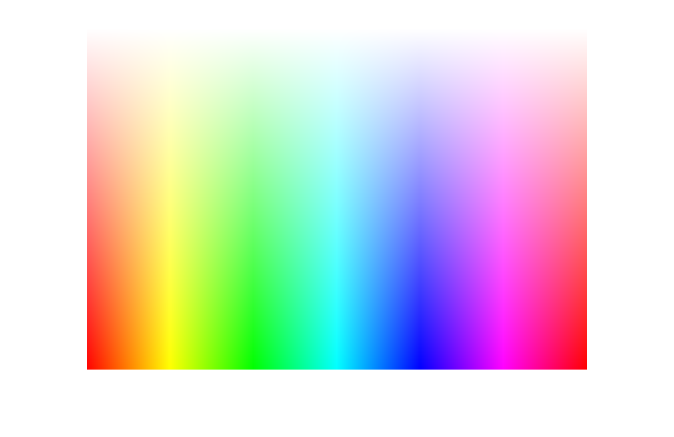
\includegraphics[width=\textwidth]{images/colourscalevhs.png}
		\caption{Illustration of HSV colour space.}
		\label{fig:colourscalehsv}
	\end{minipage}
	\begin{minipage}[t]{0.4\textwidth}
		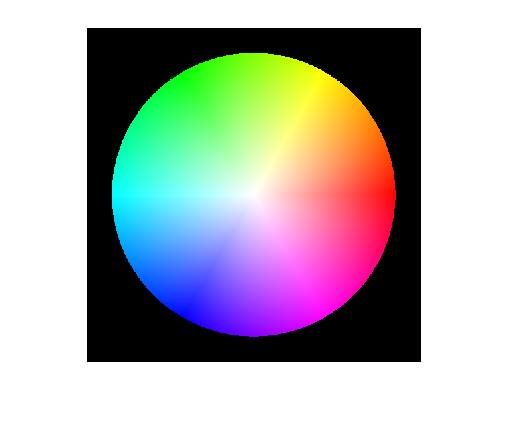
\includegraphics[width=\textwidth]{images/colourwheelvhs}
		\caption{Illustration of HSV colour space in a colour wheel.}
		\label{fig:colourwheelhsv}
	\end{minipage}
\end{figure}
As an additional illustration, the HSV colour space is represented in the colour wheel shown in figure \ref{fig:colourwheelhsv}. Inside the wheel, the saturation gradually increases from inside to outside, while the hue value depends on the angle in the circle. Inside the circle, the brightness is chosen as a constant with $V=1$, while it is set to $0$ outside, resulting in the black frame around the circle.

\subsection{PAN/XS Fusion}
A very important fact regarding multispectral images is that there is a tradeoff between spatial resolution and spetral resolution for every image, also related to the sensors. Monochromatic images only require one channel, and therefore can have a very high spatial resolution while losing spectral information since they are monochromatic. On the other hand, multispectral images need several channels to store the various colour information, which results in a loss of spatial resolution. A very important application of image processing is therefore to fuse monochromatic images of high spatial resolution with multispectral images of low spectral resolution in order to achieve a high resolution multispectral image. An example of that is presented in figures \ref{fig:hyp_lr} to \ref{fig:hrlrmixing}. Figures \ref{fig:Ipan_hr} and \ref{fig:hyp_lr} show both the initial images, where one can clearly see the difference in spatial resolution between the monochromatic and the hyperspectral image and also the difference in size of the two images. In our algorithm, the latter is resized to the size of the monochromatic one, and then additionally extended by values of the high resolution image. The resulting multispectral image is presented in figure \ref{fig:hrlrmixing}. Note, that this image should actually have the same size as the first monochromatic image. One can see that the spatial resolution of the coloured image is improved now. There are a few regions, where the information from the monochromatic image fills up elements that werer empty due to the resizing operation.

\begin{figure}[H]
	\centering
		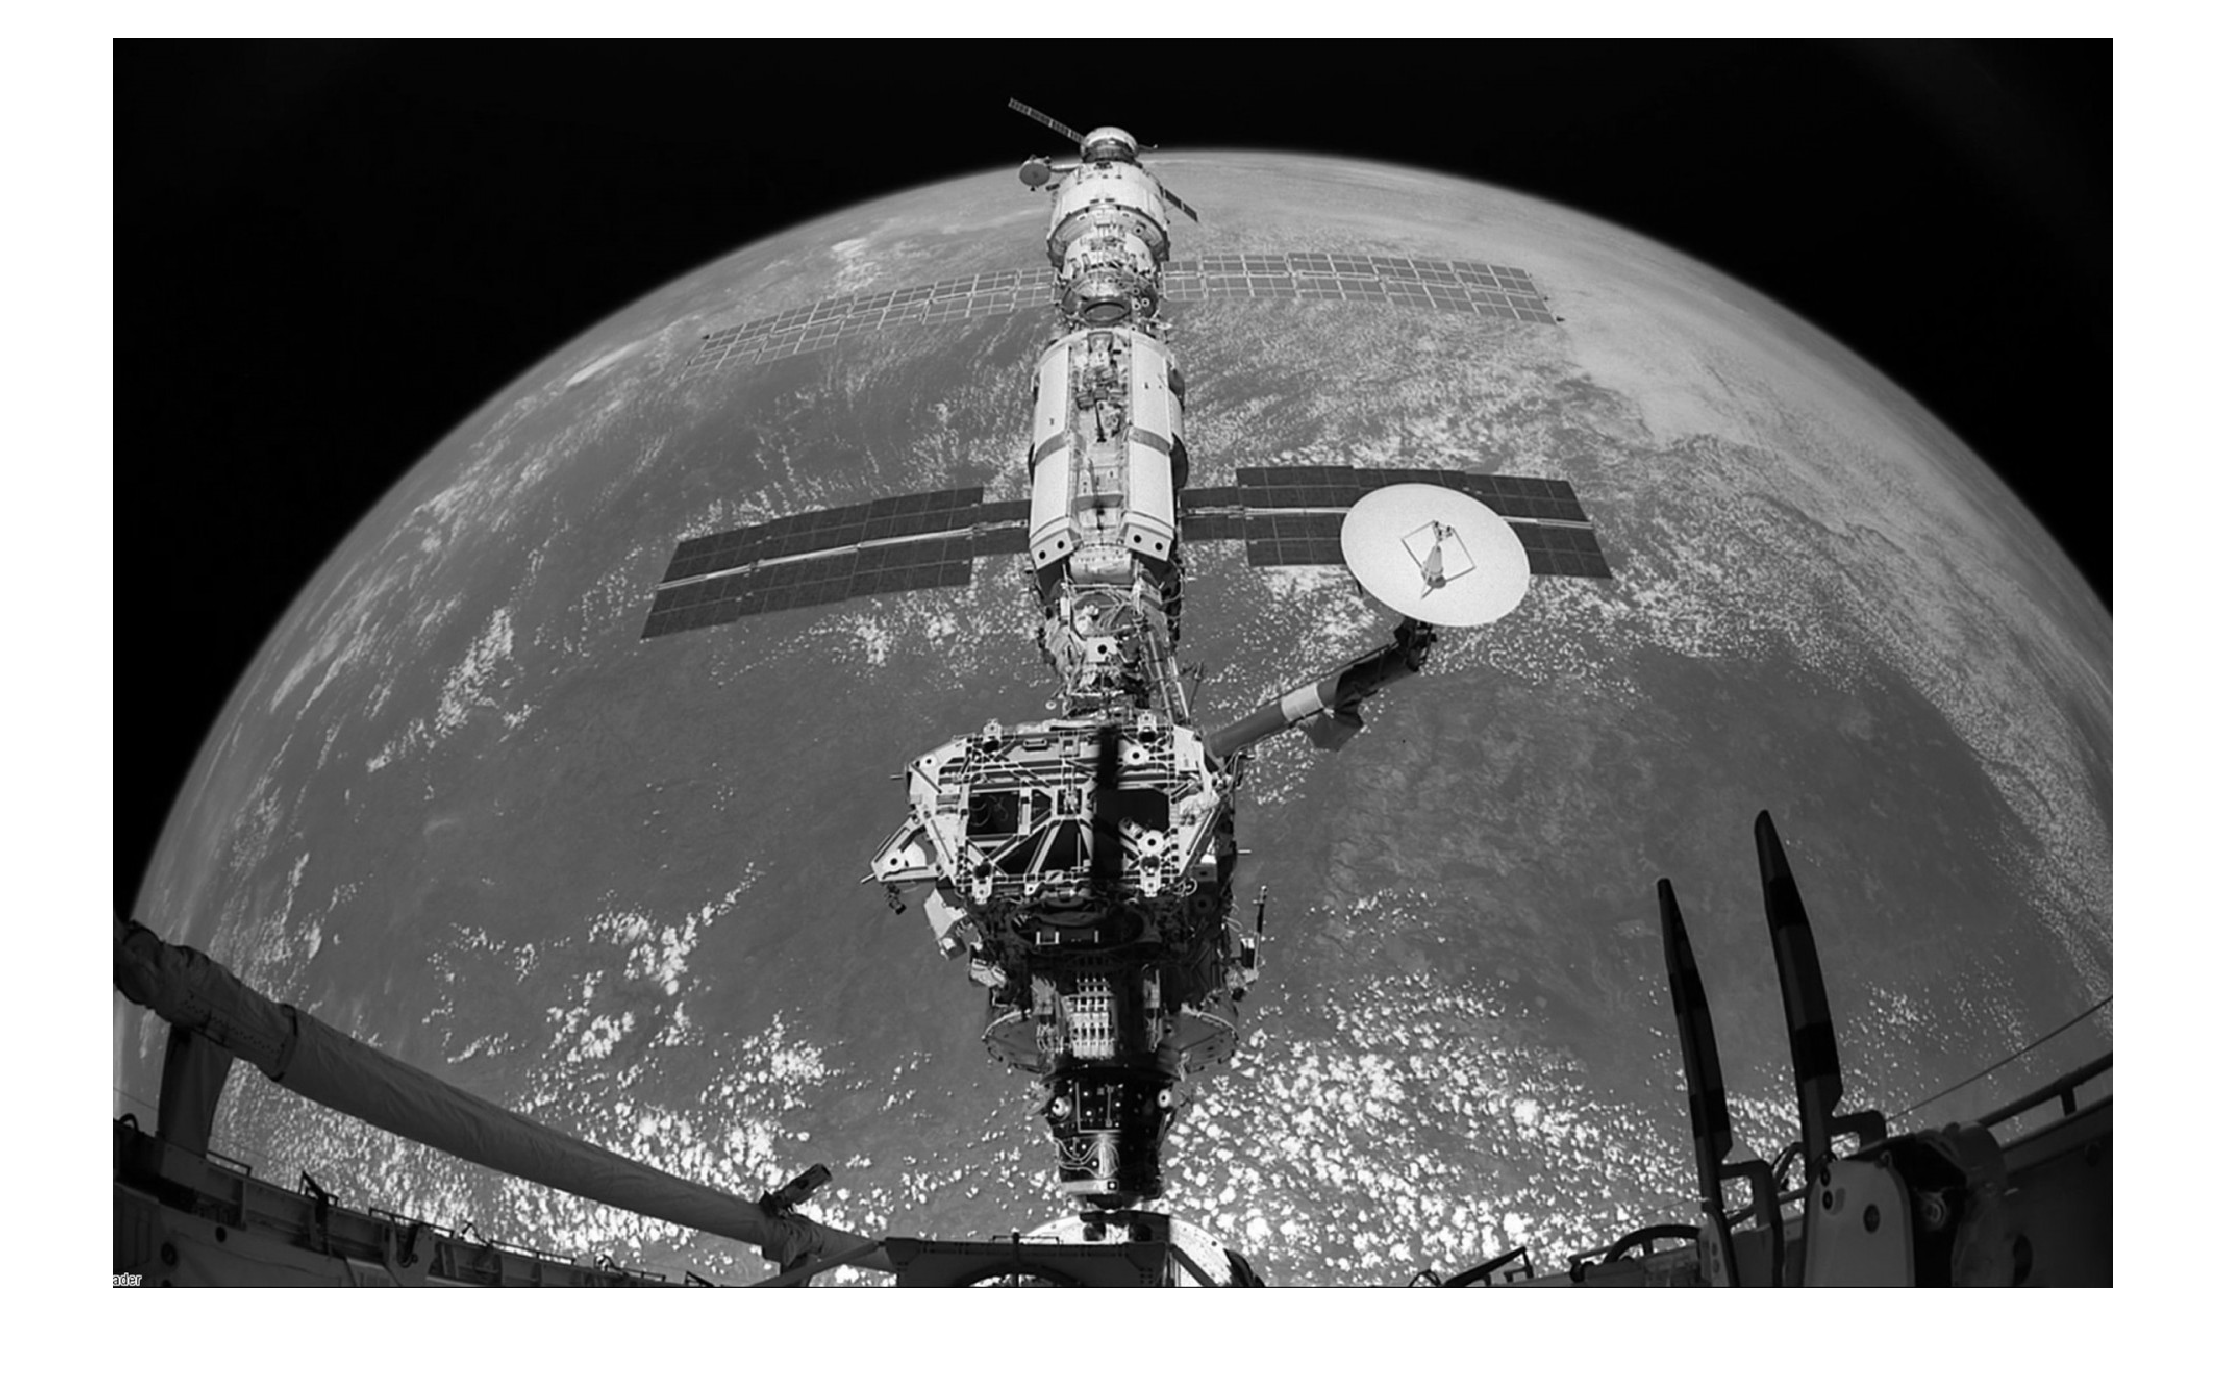
\includegraphics[scale=0.5]{images/Ipan_hr.png}
		\caption{Monochromatic image with high spatial resolution.}
		\label{fig:Ipan_hr}
\end{figure}

\begin{figure}[H]
	\centering
		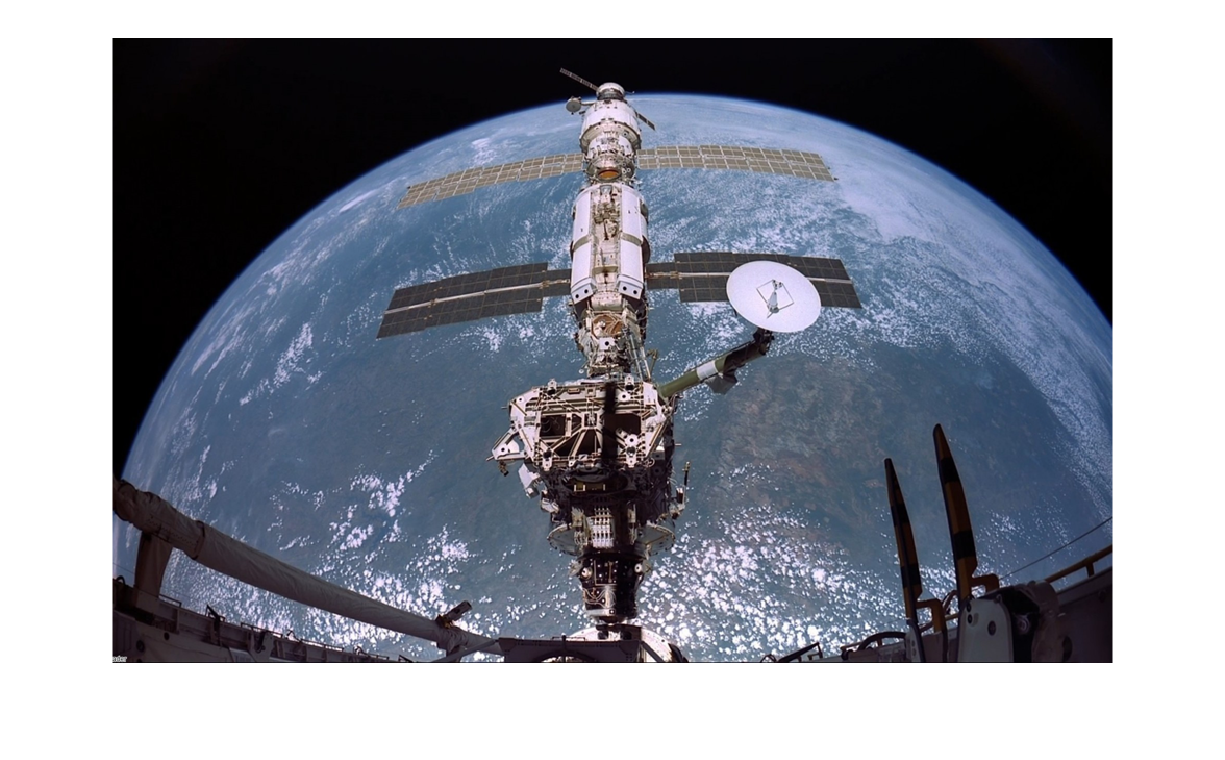
\includegraphics[scale=0.5]{images/Ihyp_lr.png}
		\caption{Hyperspectral image with low spatial resolution}
		\label{fig:hyp_lr}
\end{figure}


\begin{figure}[H]
	\centering
		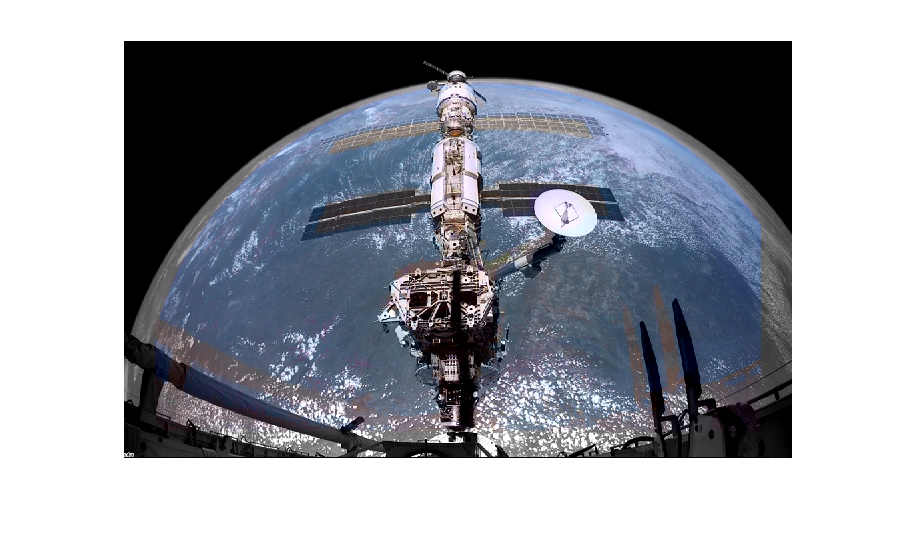
\includegraphics[scale=0.5]{images/hrlrmixing.png}
		\caption{Fused multispectral image with high spatial resolution.}
		\label{fig:hrlrmixing}
\end{figure}


\subsection{Filtering}

\subsection{Image Processing \& Analysis}

\subsection{Pattern Recognition}

\subsection{Geometry}


%%%%%%%%%%%%%%%%% TASK 3 %%%
\section{Computer Vision \& Morphology}

\subsection{Erosion \& Dilatation}

\subsection{Morphological Filtering}

\subsection{Morphological Skeletonization \& Segmentation}


%%%%%%%%%%%%%%%%% TASK 3 %%%
\section{Data Analysis \& Processing}
After having extensively discussed Image Processing and Image Analysis in the previous chapters we will now move on to Data Analysis. \\In general, Data Analysis is an extension or generalisation of Image Analysis - in particular, an image can also be seen as a set of data with a specific topology. However, data analysis is not limited to images but can be used for a vast amount of applications, be it business, science or others, where a set of data is given and information has to be extracted. Ultimately, this is the goal of data analysis: shaping, modelling and analysing the data to gain information or conclusions from given data.
Since this course puts an emphasis on analysing and processing images, all the following examples will be performed on and explained by using images as a data set.

The term \textit{data} itself can be interpreted and defined in multiple ways, which raises the need for a definition in our context of data analysis of images.
In general data can be considered as an element taken from a set of data-elements. Each data-element can then be seen as a set of different components, attributes, parameters etc. - defining what the data-element is composed of - and are often called \textit{descriptors}. Mathematically speaking, this means that our data $\boldsymbol{x}$ is associated to a vector in $\boldsymbol{\mathbb{R}^n}$ containing the descriptors,
\begin{equation*}
	x = (c_1 ... c_n)^T
\end{equation*}
which is also called the \textit{state space E} of our data.
These descriptors are the crucial part when analysing data, since they are defining a set of rules according to which we analyse the raw data.

If this terminology is applied to images, the pixels or a range of pixels in each image can be seen as such an descriptor, thus the image itself as our data-element.

\subsection{Classification}
\begin{figure}[h!]
	\centering
	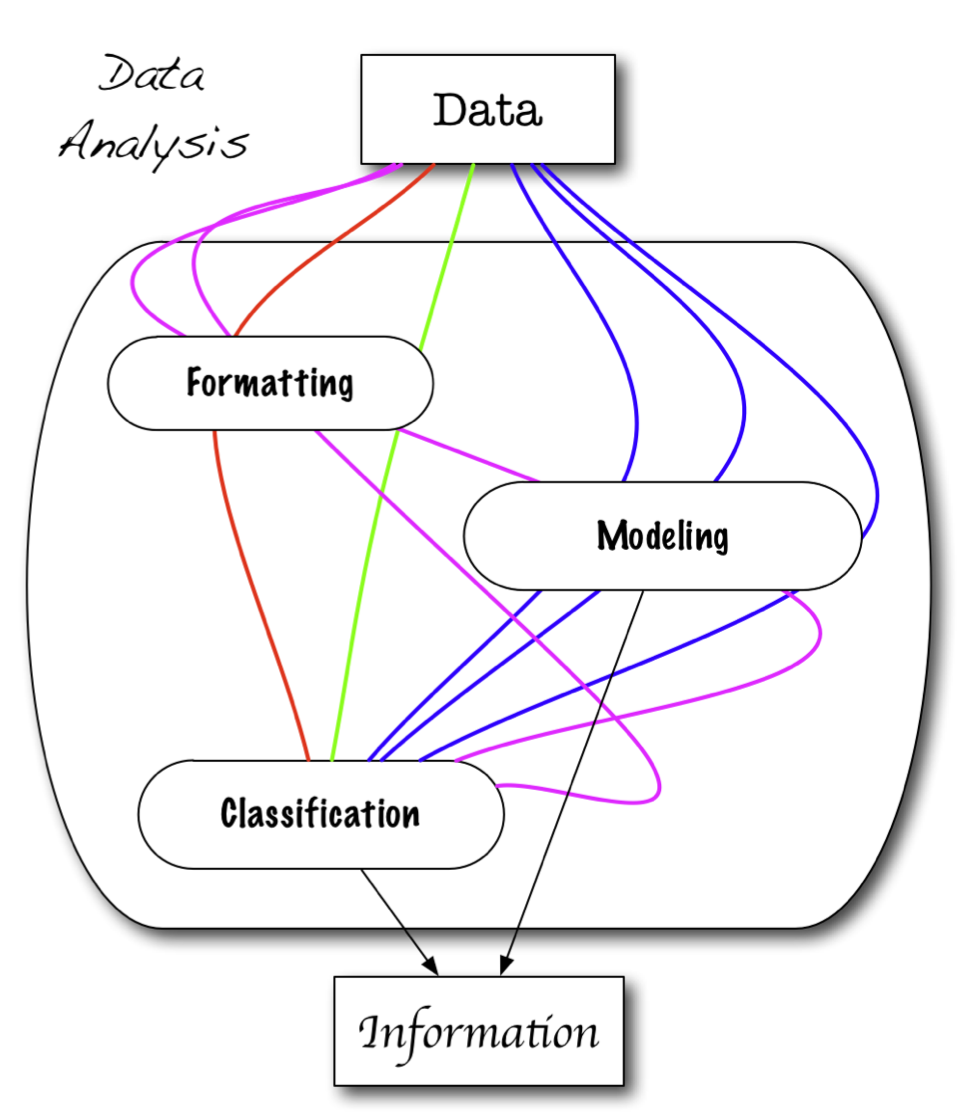
\includegraphics[width=\textwidth/2-5em]{images/data_analysis.png}
	\caption{Steps for classification \protect\footnotemark}
	\label{fig:data_anal}
\end{figure}
\footnotetext{source: lecture notes by Emmanuel Zenou}
Having a data set that consists of descriptors essentially allows us to \textit{label} this particular data set. This labelling of data is usually also described as \textit{Classification}, meaning that each data-element or sub-data-element is assigned a particular \textit{class}. In image analysis for space applications typically the pixels in an image have to be classified.

In general, classification of data consists of three steps,
\begin{enumerate}
	\item Formatting
	\item Modelling
	\item Classification
\end{enumerate}
whereas these steps are not compulsory. The formatting step usually consists of finding good descriptors, changing the state space (e.g. by re-shaping), pre-processing data (e.g. filtering) and so on.\\
The modelling step requires to find a model and its optimal parameters to fit the data, but also to fit the model output to the data and to validate the model.
In the final Classification part, the task is to find classes and a classification rule according to which distinct data will be labeled.

There are two main forms of classification, \textit{Supervised} and \textit{Unsupervised}, of which both are described and explained in detail in the following chapters.


\subsection{Supervised Classification}
Supervised Classification describes a technique, where the classes a data-set contains is known before starting the classification process. This, however, requires a human or another classification algorithm to properly detect and label desired features in either the same or similar images, which implies high effort on pre-processing and preparing the data sets.\\
For this particular technique there is a great amount of algorithms available, be it kNN, Maximum Likelihood, Bayesian or Linear Classification, Support Vector Machines or Neural Networks. During the laboratory we focused on the kNN algorithm and neural networks in particular, which is why the following sections will provide examples using these techniques.

\subsubsection{k - Nearest Neighbour}
\label{sssec:knn}
The \textit{k - Nearest Neighbour} algorithm is the most simple classification algorithm in the supervised classification domain. 

\begin{figure}[h!]
	\centering
	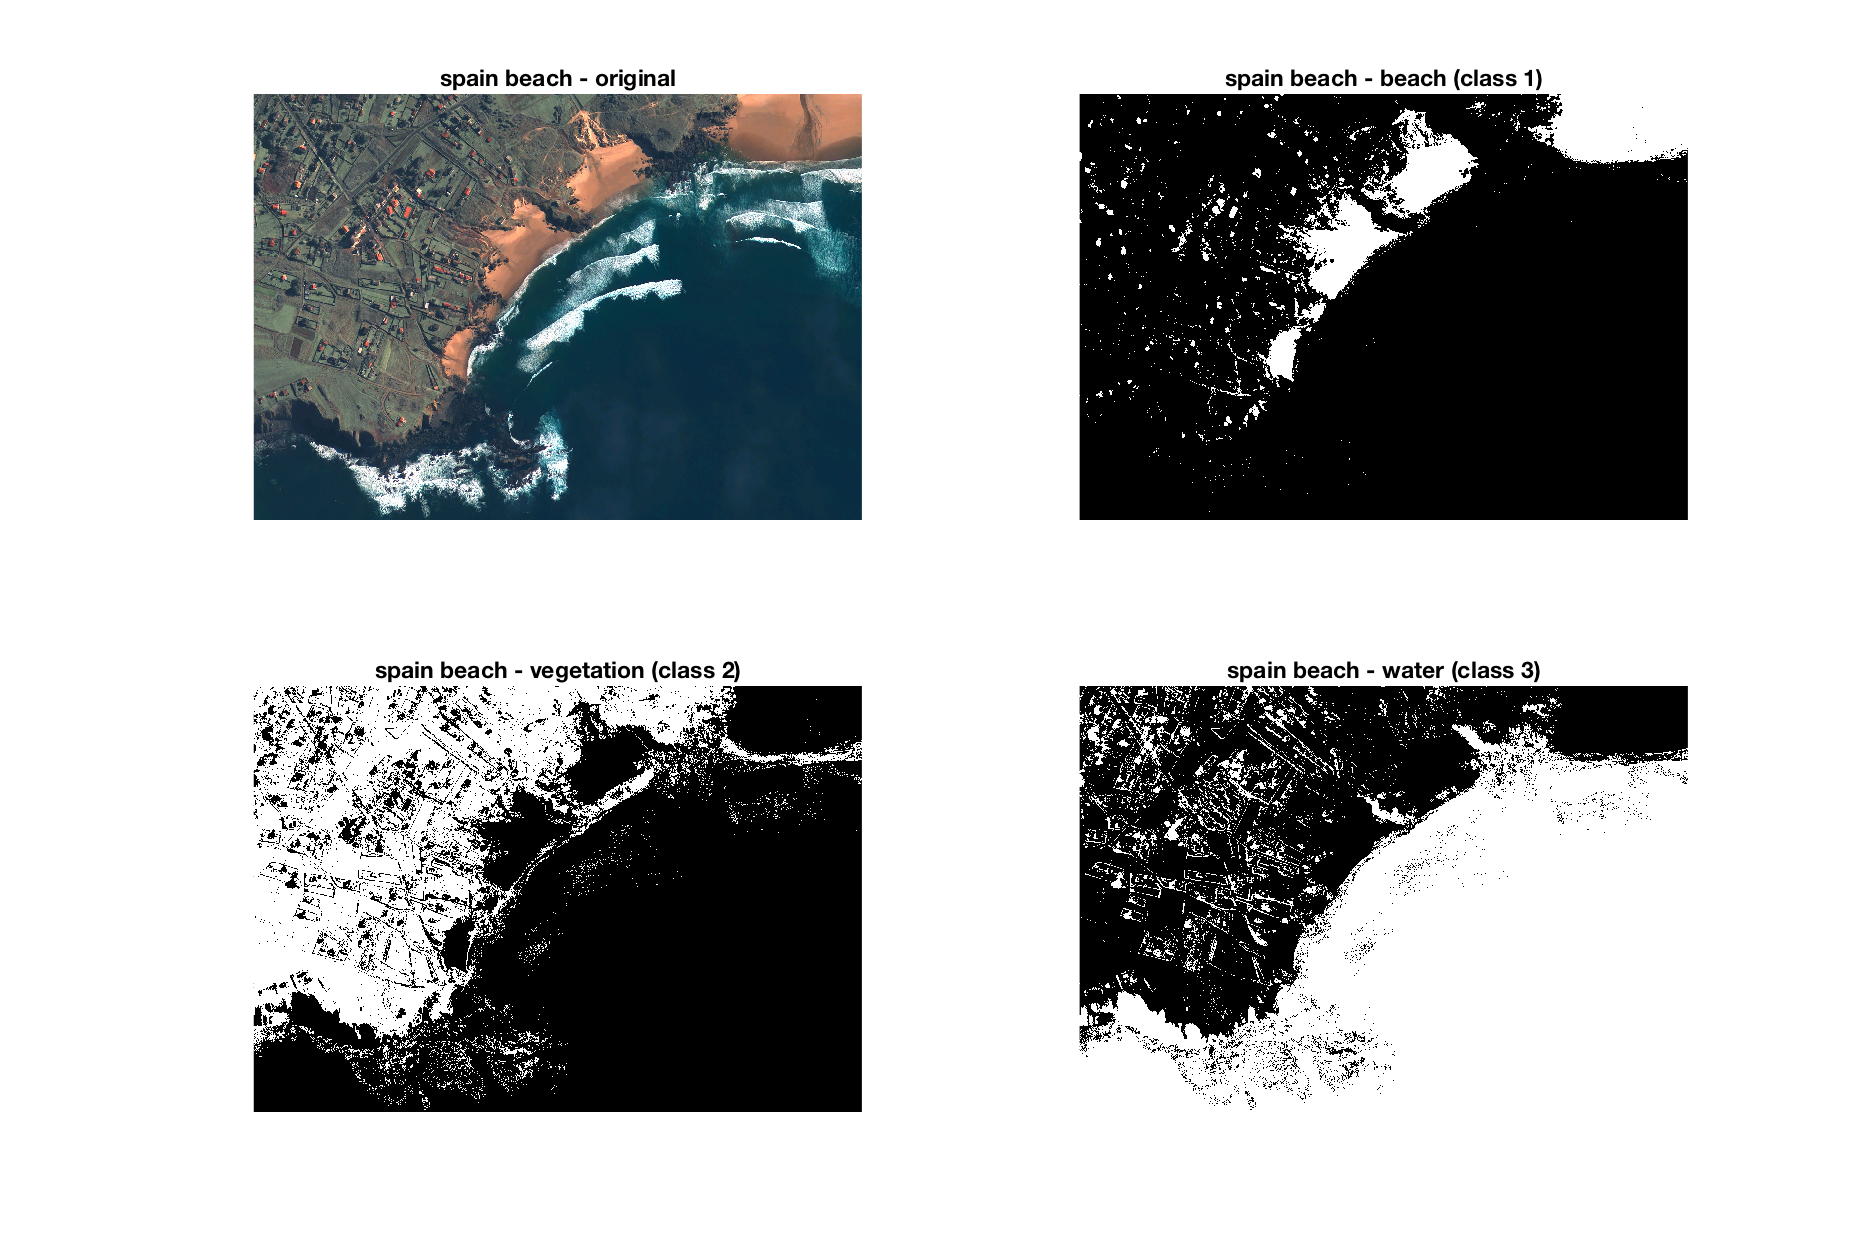
\includegraphics[width=\textwidth]{images/kNN.png}
	\caption{kNN algorithm applied on three classes}
	\label{fig:kNN}
\end{figure}

The underlying principle is to find the \textit{k} nearest neighbours to given data, to determine the class of it - which basically results in a calculation of distance. One way to apply this technique to images is to get the desired RGB values of pixels (e.g. by selecting pixels by hand at the desired image feature) and let the algorithm compare the pixels in an image to this particular RGB value.\\
This can be done of course for a range of RGB values, as is demonstrated in \cref{fig:kNN}, where an image was analysed with respect to three different classes: beach, vegetation and water. For each of these classes RGB values were taken and then used to compare the rest of the image to them. The appropriate MATLAB Code can be found in \cref{apdx:kNN}. Still, it is easy to see that this approach is not perfect. First, it requires to preprocess the image by choosing RGB values. Second, the output images are not perfect in terms of recognising the actual image features we wanted, e.g. when "detecting" water, there are a lot of points recognised on the land-part of the image, since the color is similar.


\subsubsection{Neural Networks}
A different approach of classifying data is by using neural networks. Neural Networks are layers of so-called \textit{neurons}, entities that provide a specific output given a specific input. By interconnecting those in- and outputs a network can be created.\\
But for such a network to be usable, it has to be "trained" - which means that one has to provide input and the desired output for a set of data. According to those given in- and outputs the neurons in the network are assigned a specific "weight". This is done until the desired output for a given input occurs. After that, each neuron has been assigned a weight and the neural network is ready to use.
\todo[inline]{get the matlab code running for this one}

The main advantage of neural networks is that it is very easy to use and can be very efficient. But it also has some drawbacks as one has to provide the desired outcome for input data and the whole process is relying on stochastic. 

\subsection{Unsupervised Classification}
Contrary to Supervised Classification the Unsupervised one does not need a pre-processing of data in terms of classifying example input data. The aim of Unsupervised Classification is to find classes in a given data-set (\textit{Clustering}), model the data (\textit{Regression}) and reduce the state space (\textit{Dimension Reduction}).\\
For this type of classification there is also a variety of algorithms existing, e.g. the \textit{k-Means} or the \textit{Kohonen Maps} algorithm.

\subsubsection{k-Means Algorithm} 

The k-Means Algorithm is used for Clustering given data into a previously known amount of clusters. It tries to group the data into classes, such as the sum of squared deviations is minimised. Mathematically speaking, this means minimising the cost function
\begin{equation*}
	\centering
	J = \sum_{i=1}^k \sum_{{x_j}\in{S_i}} \norm{x_j - \mu_i}^2
\end{equation*}

with $x_j$ being the distinct data points and $\mu_i$ the "Centroid" of a cluster $S_i$. This results in so-called \textit{Voronoi}-diagrams in the data space - which essentially means that the data points are divided in cells where the centroid is equally spaced with respect to the borders of the cell.\\
Applying this method on the image of the beach in Spain (see \cref{sssec:knn}), we can get a result as shown in \cref{fig:kmeans}.

\begin{figure}[h!]
	\centering
	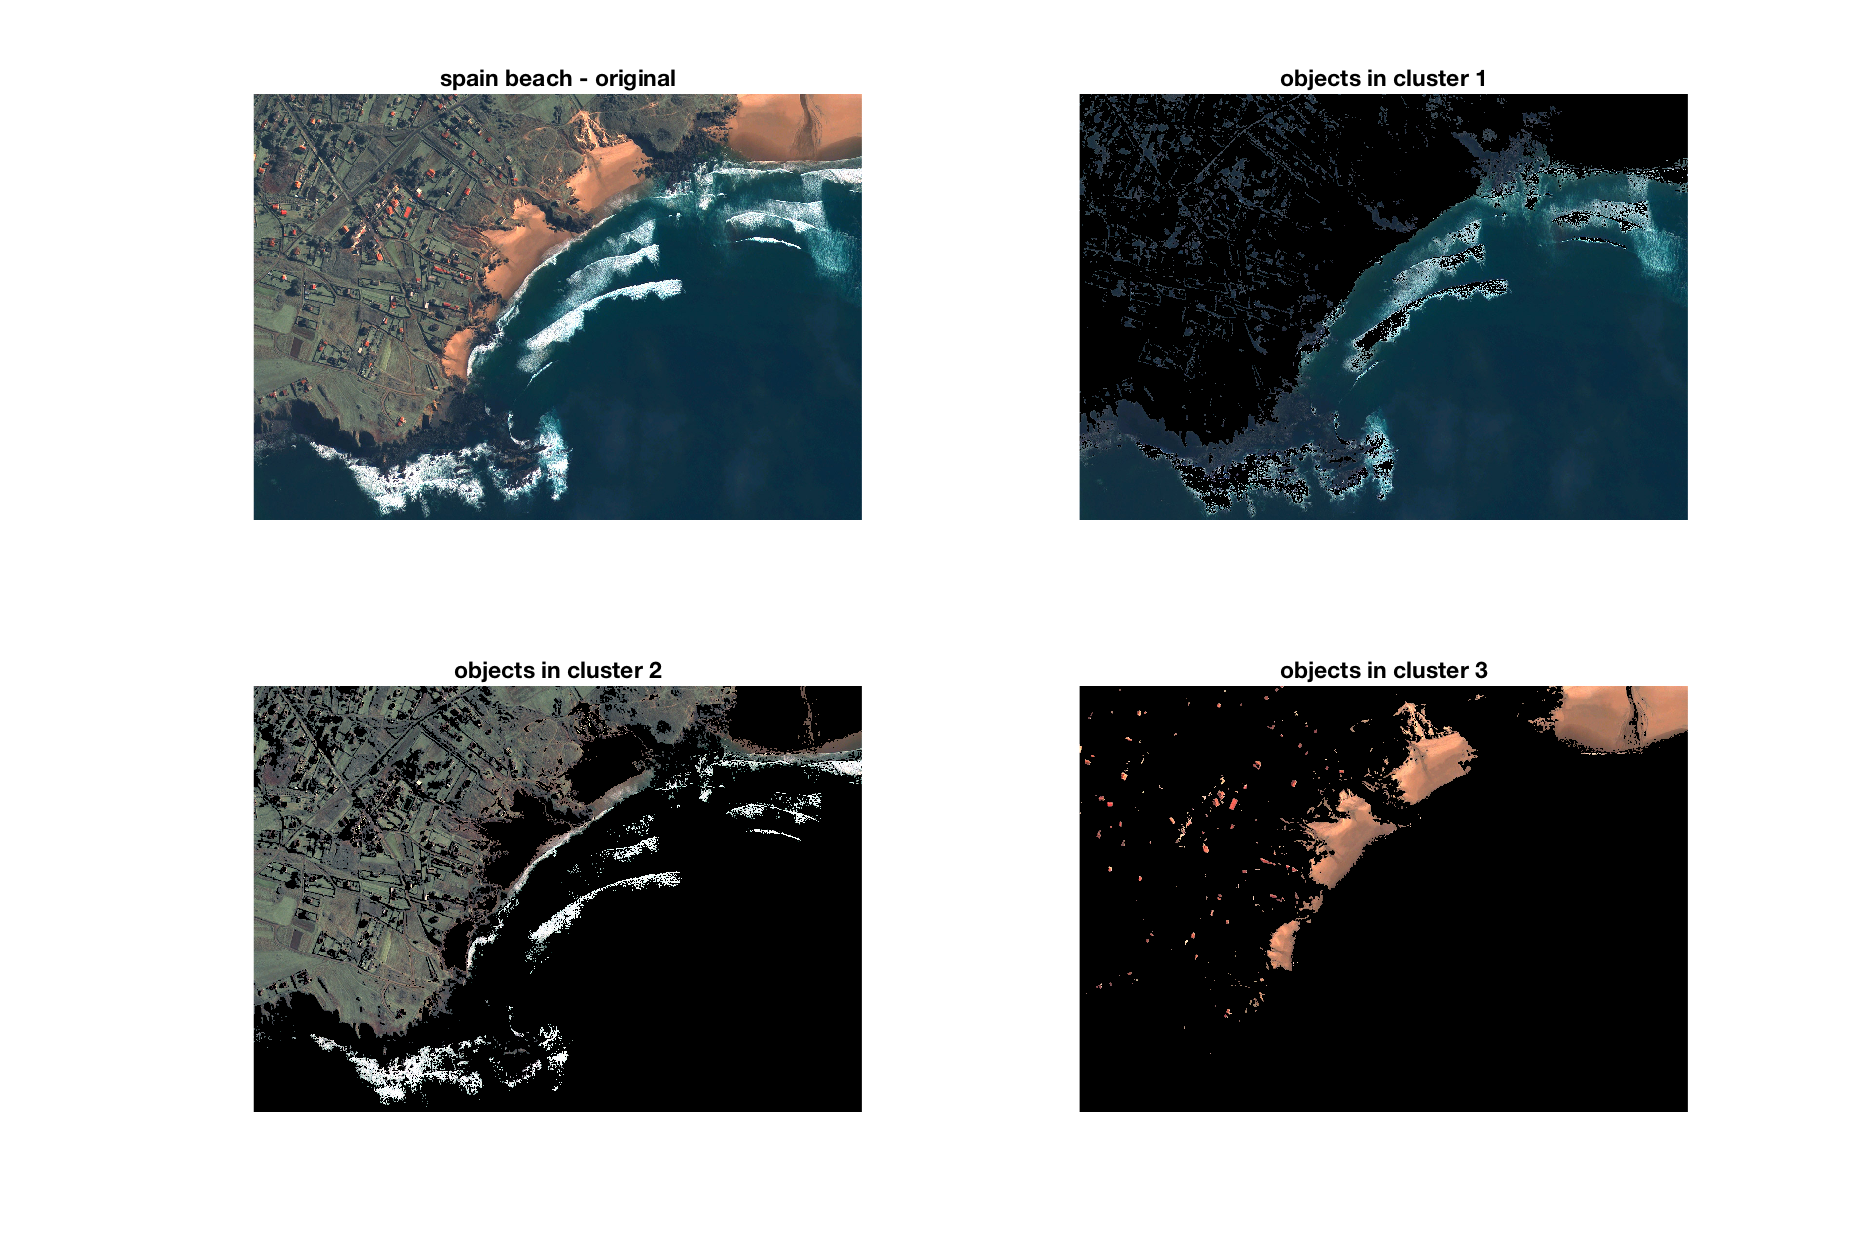
\includegraphics[width=\textwidth]{images/kMeans.png}
	\caption{k-Means Algorithm to detect three Clusters of data}
	\label{fig:kmeans}
\end{figure}

One can observe that the clustering worked very well in detecting the sea, vegetation, and beach - even though there are again some smaller errors, e.g. the beach (cluster 3) also contains rooftops of houses nearby, and the waves in the original pictures are assigned to the vegetation (cluster 2) instead of to the water (cluster 1).



\subsubsection{Dimension Reduction}
If the data to be analysed has a huge i.e. the data dimension is too big (in images this corresponds to large images), one has to reduce the data dimension to reduce the computational amount to find clusters or classes in the data. This is usually done using a technique called \textit{Principal Component Analysis} or in short PCA, where the input data is linearly mapped to new data that has a reduced state space. In practical terms this is usually done by calculating the covariance matrix and its eigenvectors. The eigenvectors corresponding to the largest eigenvalues (also called the principal components) can then be used to reconstruct a great part of the original image.
\todo[inline]{put in some MATLAB Code and images here for PCA}

%%%%%%%%%%%%%%%%%%%%%%%%%%%%%%%%%%%%%%%%%%%%%%%%%%%%%%%%%%%%%%%%%%%%%%%%%
\section{Conclusion}



% if appendix needed, uncomment the following lines
\appendix
\section{ ImProc for EO}

\section{Comp Vision and Morpho}

\section{Data Analysis}

\subsection{MATLAB Code kNN Algorithm}
\label{apdx:kNN}
\lstinputlisting{code/SupervisedClassification.m}

\subsection{MATLAB Code k-Means Algorithm}
\label{apdx:kmeans}
The Code is based on the K-Means Clustering Example in the MATLAB Documentation and can be found at \href{https://uk.mathworks.com/help/images/examples/color-based-segmentation-using-k-means-clustering.html}{uk.mathworks.com}
\lstinputlisting{code/UE34_kmeans.m}

% if bibliography needed, uncomment the following lines
%\bibliographystyle{plainnat}
%\bibliography{biblist}

%%%%%%%%%%%%%%%%% include content end %%%%%%%%%
\end{document}
